\documentclass{article}

\usepackage{siunitx} % Provides the \SI{}{} and \si{} command for typesetting SI units
\usepackage{graphicx} % Required for the inclusion of images
\usepackage{amsmath} % Required for some math elements 
\usepackage[export]{adjustbox} % loads also graphicx
\usepackage{listings}
\usepackage{matlab-prettifier}
\usepackage{float}

\usepackage{titlesec}
\usepackage{caption}
\usepackage{subcaption}


\usepackage{xcolor}

\DeclareCaptionFont{white}{\color{white}}
\DeclareCaptionFormat{listing}{%
  \parbox{\textwidth}{\colorbox{gray}{\parbox{\textwidth}{#1#2#3}}\vskip-4pt}}
\captionsetup[lstlisting]{format=listing,labelfont=white,textfont=white}
\lstset{frame=lrb,xleftmargin=\fboxsep,xrightmargin=-\fboxsep}
\titleformat{\section}[runin]
  {\normalfont\Large\bfseries}{\thesection}{1em}{}
\titleformat{\subsection}[runin]
  {\normalfont\large\bfseries}{\thesubsection}{1em}{}


\setlength\parindent{0pt} % Removes all indentation from paragraphs

\renewcommand{\labelenumi}{\alph{enumi}.} % Make numbering in the enumerate environment by letter rather than number (e.g. section 6)

%\usepackage{times} % Uncomment to use the Times New Roman font

%----------------------------------------------------------------------------------------
%	DOCUMENT INFORMATION
%----------------------------------------------------------------------------------------

\title{AMATH 353: Homework 1} % Title

\author{Trent \textsc{Yarosevich}} % Author name

\date{\today} % Date for the report

\begin{document}
\maketitle % Insert the title, author and date
\setlength\parindent{1cm}

\begin{center}
\begin{tabular}{l r}
%Date Performed: December 1, 2017 \\ % Date the experiment was performed
Instructor: Jeremy Upcal % Instructor/supervisor
\end{tabular}
\end{center}

% If you wish to include an abstract, uncomment the lines below
% \begin{abstract}
% Abstract text
% \end{abstract}

%----------------------------------------------------------------------------------------
%	SECTION 1
%----------------------------------------------------------------------------------------

\section*{Part 1.)}
\subsection*{a.)}
To create a wave moving left with speed one, I used the equation 
\begin{equation}
u(x,t) = exp(-x - ct)^2) 
\end{equation}
with $c = -1$. The following figure displays its movement to the left over time with a speed of 1.
\begin{figure}[H]
\centering
    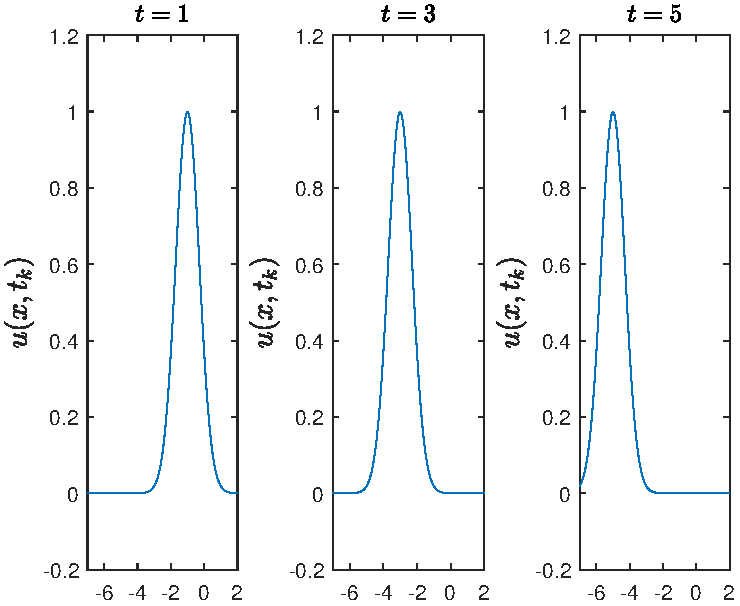
\includegraphics[width=75mm, scale=.8]{plot_1a.pdf}
	\caption{Moving left with speed 1.}
\end{figure}
\subsection*{b.) and c.)}
Parts b.) and c.) were executed with the following values for $c$ in the same equation used on part a.), which I have accompanied with visualizations. Note that the 'speed' is displayed by the identical figures and increasing or decreasing x-axes.
\begin{figure}[H]
\centering
    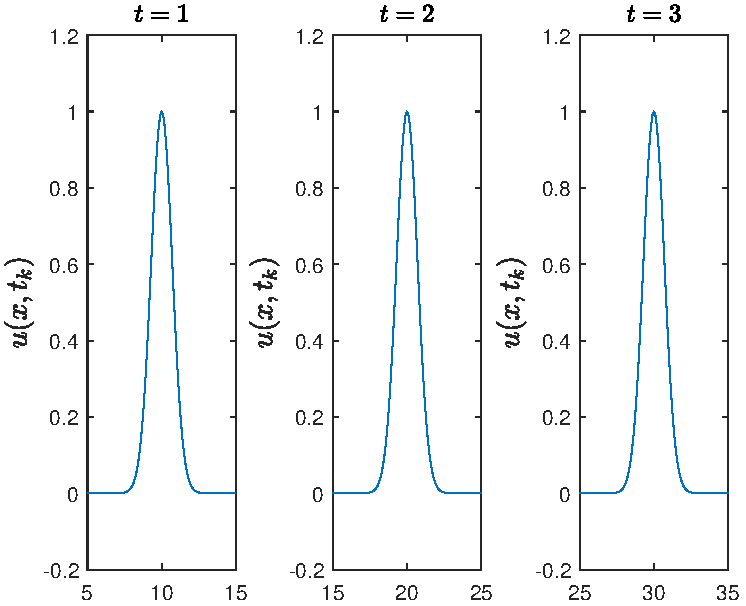
\includegraphics[width=75mm, scale=.8]{plot_1b.pdf}
	\caption{$c = 10$, moving right with speed 10.}
\end{figure}
\begin{figure}[H]
\centering
    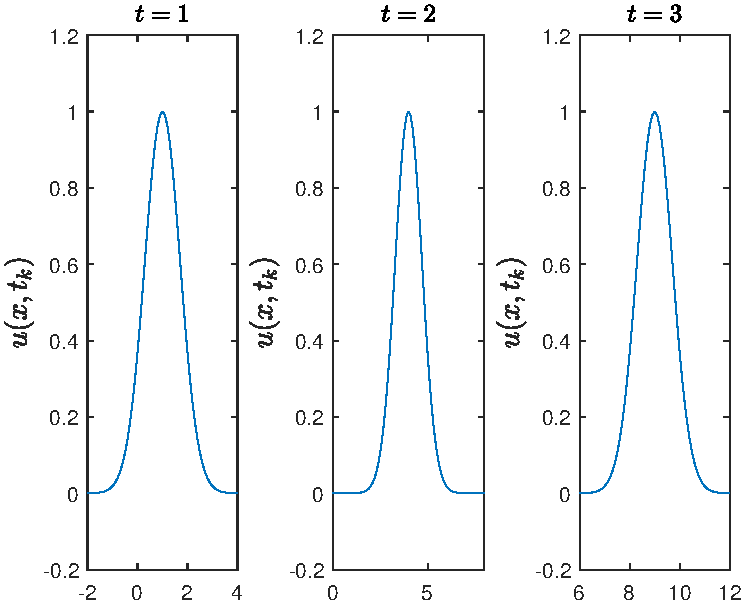
\includegraphics[width=75mm, scale=.8]{plot_1c.pdf}
	\caption{$c = t$, moving right with speed $t^{2}$.}
\end{figure}
\subparagraph*{d.)} Part d.) modifies the equation in a.) to implement decreasing amplitude inversely proportional to $t$.
\begin{equation}
u(x,t) = \frac{1}{t}exp(-x - ct)^2) 
\end{equation}

\begin{figure}[H]
\centering
    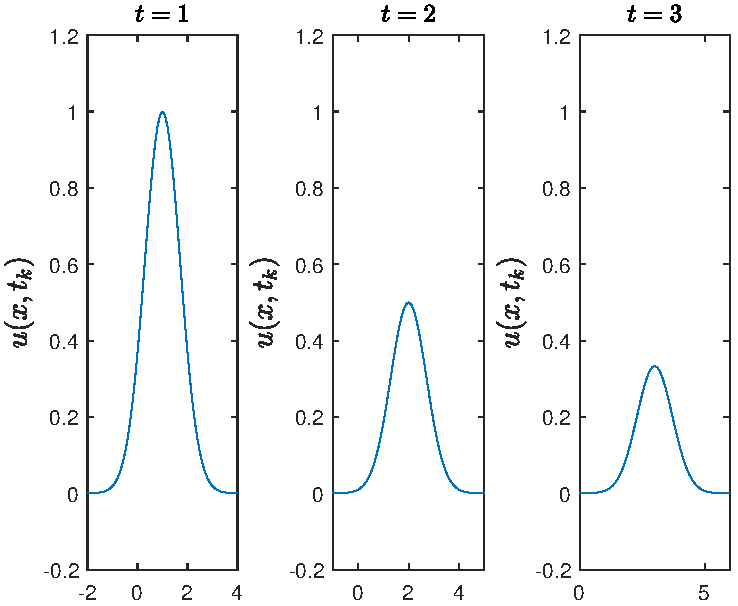
\includegraphics[width=75mm, scale=.8]{plot_1d.pdf}
	\caption{$c = 10$, moving right with speed 1 and amplitude inversely proportional to $t$.}
\end{figure}
\section*{Part 2.)}
\subsection*{a.)} 
$v_{tt} - v_{xxx} = 0$
\subsection*{b.)}
Let $\alpha = \beta = 1$\\

\noindent By linear differential operators, 
\begin{equation}
\begin{aligned}
u_{3, tt} = u_{3, xxx} \\
(u_{1} + u_{2})_{tt} = (u_{1} + u_{2})_{xxx}\\
u_{1, tt} + u_{2, tt} = u_{1, xxx} + u_{2, xxx}\\
u_{1, tt} + u_{2, tt} - u_{1, xxx} - u_{2, xxx} = 0\\
u_{1, tt} - u_{1, xxx} + u_{2, tt} - u_{2, xxx}) = 0\\
\end{aligned}
\end{equation}
Thus as hoped after plugging in $u_{3}$ we arrive at the sum of two homogeneous equations of the solutions $u_1$ and $u_2$.

\end{document}